
\section{Lecture 13: Equation of motion for simple harmonic oscillators}

The lecture begins with what is really a review of gravitational potential energy, which is still certainly worth watching, to make sure that you everything everything clearly. In addition, the explanation for the potential energy (below) is compared to gravitational potential energy.

First, the potential energy of a spring is derived, which I did in homework 4 (week 5), problem 5.

As a quick refresher: we set $x = 0$ at the relaxed length of the spring, and extend it a distance $x$ further. The spring force is $-k x$, and the force we need to provide to overcome that is $+ k x$. The work we do in extending the spring is all stored as potential energy in the spring, so

\begin{equation}
U_{spring} = W = \int_0^x k x \mathop{dx} = \Big[\frac{1}{2} k x^2\Big]_0^x = \frac{1}{2} k x^2
\end{equation}

It follows, then, that $U_{spring} = 0$ at $x = 0$. As usual, we can define this however we want, but any other definition would only cause problems in most cases, and therefore be silly to make.

As is the case with gravity, as stated in the beginning of the lecture (of which I took no notes), the force is always in the direction \emph{opposite} that of increasing potential energy. For gravity, this turns out to be an always-attracting force. For springs, this turns out to be a restoring force: if you stretch the spring, the force is always such that it pulls to spring back together. If you instead compress the spring, the force reverses, and now tries to push it back to its original length. In both these cases, the force is in the opposite direction of increasing potential energy, since potential energy increases both when the spring is compressed and when it is extended.

Let's now look at the reverse situation. Can we go from knowing only the potential energy, to finding the spring's force? Yes, we can, and it's very easy: we take the derivative of the potential energy, with respect to $x$:

\begin{align}
U &= \frac{1}{2} k x^2\\
\frac{dU}{dx} &= + k x = - F_{sp}\\
\frac{dU}{dx} &= -F_x
\end{align}

Since the force is one-dimensional, we can write $F_x$ for the force. The minus sign is important, and means what we mentioned above: the force is in the direction \emph{opposite} the increase in potential energy. If $\frac{dU}{dx}$ is positive, you are moving in that direction, and you get a minus sign for the force -- it is opposite our motion, since the motion is towards increasing potential energy.\\
If $\frac{dU}{dx}$ is negative, we are moving towards decreasing value of potential energy, and the force is positive (in the same direction as the $x$ motion).

In multiple dimensions, we can find a similar result. If we know the potential energy as a function of $x$, $y$ and $z$, we can find the force components along each axis by taking partial derivatives. So given $U(x, y, z)$, we can find force components $F_x$, $F_y$ and $F_z$:

\begin{align}
\frac{\partial U}{\partial x} = - F_x\\
\frac{\partial U}{\partial y} = - F_y\\
\frac{\partial U}{\partial z} = - F_z
\end{align}

Partial derivatives are quite simple; you calculate them for one function argument at a time. So you essentially first find $\displaystyle \frac{d}{dx} U(x,y,z)$, while \emph{treating y and z as constants}; that gives you the negative of the force along the $x$ axis.\\
In other words, as an example:

\begin{equation}
\frac{\partial}{\partial x}\left(2x^2 - 3y + 2 x y - 3z\right) = 4x + 2y
\end{equation}

The $-3 y$ term disappears, since we consider it constant. Likewise, $2 x y$ becomes $2 y$, since $\displaystyle \frac{d}{dx}(2 x y) = 2 y \frac{d}{dx} (x)$ if $y$ is a constant. Similarly, the $z$ term disappears, since we treat it as a constant.\\
If this polynomial was $U(x, y, z)$, then we just found $-F_x = 4x + 2 y$, so $F_x = -4 x - 2 y$.

You then simply repeat the process for the $y$ and $z$ components, keeping the other two axes constant, and you are done.

Two more realistic examples are covered in the lecture. First, for one-dimensional gravitational potential energy:

\begin{align}
U &= + m g y \text{ (with +y upwards)}\\
\frac{dU}{dy} &= m g\\
F_y = -\frac{dU}{dy} &= - mg
\end{align}

And indeed, the gravitational force is $- m g$, assuming increasing $y$ is upwards.

Next, another one-dimensional problem of gravitational potential energy, this time in general, rather than very close to Earth's surface:

\begin{align}
U &= -\frac{M m G}{r} \text{ (where $M$ is the mass of the Earth)}\\
\frac{dU}{dr} &= +\frac{M m G}{r^2}\\
F_r = -\frac{dU}{dr} &= -\frac{M m G}{r^2}
\end{align}

Again, we find a familiar result.

\subsection{Stable and unstable equilibrium}

Next up, let's look at equilibrium. Say we have a surface, that may look like this:

\begin{center}
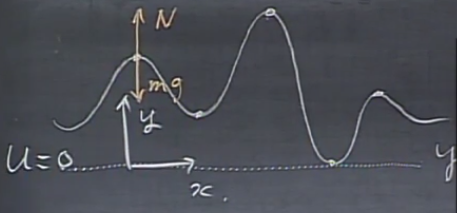
\includegraphics[scale=0.8]{\pIImages/lec13_equilibrium}
\end{center}

The points along the curve have a gravitational potential energy which is $U = m g y$, since we defined $U = 0$ at $y = 0$ (the $= 0$ part is just outside the screen grab above). Since the plot is of $y = f(x)$, for some function $f$, we can also write that $U = m g f(x)$.

There are then points along this curve where $\displaystyle \frac{dU}{dx} = 0$. Those points occur where the curve's slope (or derivative) are zero, by definition, which is at the top of each peak, and at the bottom of each valley, as signified by a dot in the above figure.

From the definition we found before, that then means that $-F_x = 0$, so the net force in the $x$ direction is zero.\\
At such a point, there is a force $-m g$ in the $y$ direction, and a normal force $N = + m g$, so that there is no net force there, either.

Since there is no net force on the object at one of these points, and we can put it in such a situation at rest, it will stay exactly where it is.\\
However, there is an important difference between these two types of points  (peaks and valleys). If we try to balance a marble at the top of such a peak, just about any tiny vibration, small amount of wind etc. will get it moving. Being at the top of a large downwards slope, in either direction, it will then clearly begin to accelerate downwards -- and again, the force is in the direction of decreasing potential energy (which of course is the same thing as being in the \emph{opposite} direction as \emph{increasing} potential energy).

However, if we put a marble in one of the valleys, what happens? If there is a small force, causing a motion in any direction, it will be forced back into the valley. The force is yet again in the direction opposing the increase in potential energy, and potential energy increases both to the left \emph{and} to the right! Therefore, the force is such that the marble is returned to the middle of the valley again, to the point of lowest potential energy.

The difference between these two zero points are that the peaks provide \emph{unstable equilibrium}, while the valleys provide \emph{stable equilibrium}. If there is a disturbance in the first case, it goes out of control. In the second case, in the valleys, any small disturbance is automatically countered, and the object goes back to where it was, at the bottom.

We can find out which of these two cases a point is mathematically, by looking at the second derivative. If the second derivative of potential energy with respect to $x$ is positive, it's a point of stable equilibrium. If it is negative, it's instead a point of unstable equilibrium.

\subsection{Another look at a spring oscillator}

Let's have another look at the oscillation of a mass on a spring, this time from an energy perspective. We know that $\displaystyle U = \frac{1}{2} k x^2$, so a plot of $U(x)$ would be a parabola:

\begin{center}
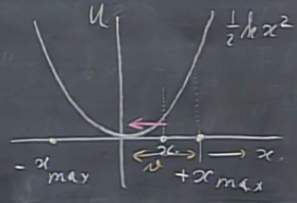
\includegraphics[scale=0.8]{\pIImages/lec13_spring_pe}
\end{center}

Say we have a mass attached to a spring, as usual, and we extend it to $x_{max}$, and let it go, with zero speed.

We know that it will oscillate between $+x_{max}$ and $-x_{max}$, but we can now gain a second insight into this oscillation (albeit one mentioned earlier). Say we release the mass at an extension $x_{max}$ beyond the spring's natural length. That means the potential energy in the spring at that time is

\begin{equation}
U_{initial} = \frac{1}{2} k x_{max}^2
\end{equation}

Since we know that the force will be in the direction opposing the increase in potential energy, the mass will be pulled inwards, towards $x = 0$. Once it crosses the zero point, the force switches directions, since the current \emph{velocity} vector is towards increasing potential energy (the spring is being compressed to be shorter than its natural length). That means the force (and thus the acceleration) instantly flips over, and the mass starts slowing down. The new force is once again in the direction opposing the increase in potential energy, which is again towards $x = 0$, which is now towards the right in the figure.

Because spring forces are conservative (for ideal springs), we can use conservation of energy to write an equation for this system. The \emph{total} energy in the system must equal the spring's stored potential energy at $t = 0$, plus the mass's kinetic energy at $t = 0$. The latter is zero, since we release it at rest (zero speed), so $E_{total} = U_{initial}$. That energy must be held constant -- conservation of energy. Therefore, the sum of the mass's kinetic energy $\displaystyle \frac{1}{2} m v^2$ and the spring's stored energy $\displaystyle \frac{1}{2} k x^2$ must always equal that initial energy. We can set up an equation for this:

\begin{equation}
\frac{1}{2} m v^2 + \frac{1}{2} k x^2 = \frac{1}{2} k x_{max}^2
\end{equation}

This equation must \emph{always} hold for this system, unless there are other forces, such as friction, which we ignore for now.\\
Because $v = \dot{x}$, we can rewrite this equation a bit, by making that substitution, and getting rid of all of the one-halves, and dividing through by $m$:

\begin{align}
\frac{1}{2} m \dot{x}^2 + \frac{1}{2} k x^2 = \frac{1}{2} k x_{max}^2\\
\dot{x}^2 + \frac{k}{m} x^2 - \frac{k}{m} x_{max}^2 = 0
\end{align}

We can then take the time derivative of this. Keep in mind that since the equation is in terms of $x$, we need to use the chain rule for most terms.

\begin{align}
\frac{d}{dt} \left(\dot{x}^2 + \frac{k}{m} x^2 - \frac{k}{m} x_{max}^2\right) = \frac{d}{dt} (0)\\
2 \dot{x} \ddot{x} + 2 \frac{k}{m} x \dot{x} - 0 = 0
\end{align}

We can simplify this equation by dividing through by $2 \dot{x}$:

\begin{equation}
\ddot{x} + \frac{k}{m} x = 0
\end{equation}

Isn't it remarkable? We get the equation for simple harmonic motion, and so we find the same old solutions:

\begin{align}
x        &= x_{max} \cos(\omega t + \varphi)\\
\dot{x}  &= - \omega x_{max} \sin(\omega t + \varphi)\\
\ddot{x} &= - \omega^2 x_{max} \cos(\omega t + \varphi) = -\omega^2 x\\
\omega  )    &= \sqrt{\frac{k}{m}}\\
T           &= \frac{2 \pi}{\omega} = 2 \pi \sqrt{\frac{m}{k}}
\end{align}

\subsection{Motion of a ball along a circular track}

Say we have a circular (or at least semicircular) track of radius $R$. We define $y = 0$ and $U = 0$ to be at the bottom of the track.

\begin{center}
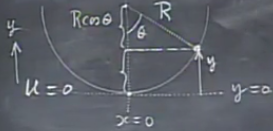
\includegraphics[scale=0.8]{\pIImages/lec13_bowl}
\end{center}

When the ball is at some random location $y$, we can find the angle made with the vertical, $\theta$, via trigonometry.\\
First, we find that the radius $R$ acts as the hypotenuse of a right triangle, where the $x$ component $R \sin \theta$ is at the bottom, and the left side has height $R \cos \theta$. Note that the $y$ coordinate fits $y = R - R\cos \theta$, so that $y = R (1 - \cos \theta)$.

With that in mind, we can write $U$ as a function of the angle $\theta$ now:

\begin{equation}
U = m g y = m g R (1 - \cos \theta)
\end{equation}

Notice that at $\theta = 0$, $U = 0$, as we defined.\\
At $\displaystyle \theta = \frac{\pi}{2}$, $U = m g R$, since it is a height $R$ above $y = 0$.

Using the definition of a radian as the arc length subtended by an angle, where $dS$ is the arc length and $d\theta$ the angle, we find

\begin{align}
\frac{dS}{R} &= d\theta\\
dS &= R d\theta
\end{align}

Taking the time derivative of both sides, we find

\begin{equation}
\frac{dS}{dt} = R \frac{d\theta}{dt} = R \dot{\theta}
\end{equation}

The left-hand term is just the distance moved per unit time, so $\displaystyle \frac{dS}{dt} = v = R \dot{\theta}$.

In most cases, we use $\displaystyle \omega = \dot{\theta} = \frac{d\theta}{dt}$, but in most cases, $\omega$ is also a constant. In this case, it is a function of the angle; the angle will change the fastest near $\theta = 0$ (at the bottom), where the speed is at a maximum, while it will change slower as the ball climbs up the ``edges'' of the circle (I think of it as a ``two-dimensional bowl''), as it is about to come to a halt, and change direction.

As a short aside, we can, as a small-angle approximation, use

\begin{equation}
\cos \theta \approx 1 - \frac{\theta^2}{2}
\end{equation}

This approximation uses the first two terms of a Taylor expansion for $\cos \theta$. If you are unfamiliar with Taylor expansions, you could look them up (even the basics are a bit too much to cover in what is already an aside). In short, they provide for a way to approximate about any function as a polynomial, or -- with an infinite amount of terms -- exactly equal those functions.

Last time we used such an approximation, we used only the first term, $\cos \theta \approx 1$. That's too inexact for this case, though -- we would end up with $U = m g R (1 - 1) = 0$ for all $\theta$!

Even for angles of about 11.5 degrees, the error caused by this approximation is way, way less than 1\% (less than 0.01\%, actually). In fact, for as much as 30 degrees, we have $\cos(\ang{30}) \approx 0.8660254$, while the approximation gives $0.862922$. It's off by about 0.3\% -- still not a lot, all things considered.

Let's return to the problem at hand. Using this approximation, we apply the conservation of mechanical energy to this system. The total mechanical energy must be a constant. If we release the object as zero speed, and thus zero kinetic energy, the total energy (kinetic + potential) must always equal that value:

\begin{equation}
M_E = \frac{1}{2} m v^2 + m g R(1 - \cos \theta)
\end{equation}

Since $v = R \dot{\theta}$, $v^2 = R^2 \dot{\theta}^2$. Let's also apply our approximation for the cosine. What we end up with is

\begin{align}
M_E &= \frac{1}{2} m R^2 \dot{\theta}^2 + m g R(1 - (1 - \frac{\theta^2}{2}))\\
M_E &= \frac{1}{2} m R^2 \dot{\theta}^2 + m g R \frac{\theta^2}{2}
\end{align}

We can now take the time derivative of this. $M_E$ is a constant, so that becomes zero. As far the rest, we use the chain rule again:

\begin{align}
0 &= \frac{1}{2} m R^2 (2 \dot{\theta} \ddot{\theta}) + \frac{m g R}{2} 2 \theta \dot{\theta}\\
0 &= m R^2 \dot{\theta} \ddot{\theta} + m g R \theta \dot{\theta}\\
0 &= R^2 \ddot{\theta} + g R \theta
\end{align}

We can rearrange that as

\begin{equation}
\ddot{\theta} + \frac{g}{R} \theta = 0
\end{equation}

... and it is then again obvious that we have as simple harmonic oscillator! We know the solution to this differential equation, so we can write down

\begin{align}
\theta &= \theta_{max} \cos (\omega t + \varphi)\\
\omega &= \sqrt{\frac{g}{R}}\\
T      &= 2 \pi \sqrt{\frac{R}{g}}
\end{align}

Note that this $\omega$ is completely unrelated to the $\displaystyle \frac{d\theta}{dt}$ we had earlier in the derivation -- it's a good thing we didn't call that $\omega$! This one is a constant, while the other one changed with time.

Note how these equations are identical to the ones for a pendulum, that we derived earlier, also using a small-angle approximation. This time, however, it is our approximation which caused the similarity -- we made the equation quadratic in $\theta$ by doing that. The spring oscillation was quadratic in $x$ from the beginning.

Finally, on to an important detail. Nowhere in this derivation did we consider the normal force from the track on the ball. Is it really safe to ignore it? Why?

It turns out that yes, we can ignore it, because in the case of this circular track, it is always perpendicular to the direction of motion. A force perpendicular to a motion \emph{cannot} do work, because of the definition of the dot product: an angle of $\ang{90}$ between force and displacement always means zero work.

Next, a very interesting demonstration follows, that might cause some sleeplessness until we find the answer to what's going on, likely in two weeks or so.

\section{Lecture 14: Orbits and escape velocity}

As we know, the gravitational force has infinite range. Its strength at a distance is limited, though, due to the inverse square relationship. Because of this, there is a speed, the \emph{escape velocity}, that lets you escape from a body's gravitational field. That is, if you start out with that speed, you will escape it forever, even with no additional outwards force (no engines required). Of course, if you \emph{do} have engines, you certainly don't need to stay above the escape velocity the entire time to get away; all you need to do is overcome the force of the gravitational pull.

We can find this velocity for a given body (such as the Earth) quite easily, using conservation of energy. The kinetic energy at launch must be $\displaystyle \frac{1}{2} m v_{esc}^2$, and since the problem definition is that in never adds to that kinetic energy (no engines). That must therefore be the total energy of the object, at all times. The total energy at any given time is the sum of the kinetic energy at some point $r$, which we call $\displaystyle \frac{1}{2} m v_r^2$, and the potential energy at that point, $\displaystyle - \frac{G M m}{r}$, with $M$ being the mass of the Earth (or the body), and $m$ the mass of the object trying to escape.

\begin{equation}
\frac{1}{2} m v_{esc}^2 + \left(-\frac{G M m}{R_{Earth}}\right) = \frac{1}{2} m v_r^2 + \left(-\frac{G M m}{r}\right)
\end{equation}

On the left side, we have the total energy as we start out our journey, and on the right, the total energy some distance $r$ away.

However, since the goal is for the energy to be enough to escape to an infinite distance, the kinetic energy ``at'' infinity (let's just say extremely, extremely far away, since being ``at'' infinity is meaningless), the potential energy is zero, by definition. The kinetic energy is also zero, \emph{if} we gave it \emph{just} enough energy, and not any more than required (we know that the Earth's gravity will reduce the speed, and thus the kinetic energy, as time goes on).

Because of this, we can set the entire right side of the equation equal to zero, which is valid ``at'' infinity (or just so far away that the gravitational pull of the Earth is now completely negligible), and solve for the escape velocity:

\begin{align}
\frac{1}{2} m v_{esc}^2 -\frac{G M m}{R_{Earth}} = 0\\
v_{esc}^2 -\frac{2 G M}{R_{Earth}} = 0\\
v_{esc} = \sqrt{\frac{2 G M}{R_{Earth}}}
\end{align}

where, again, $M$ is the mass of the Earth. For Earth, this value is then about 11.2 km/s. So if we neglect air resistance, which will surely make these results valid if we are at the Earth's surface, if we could fire a cannon ball at more than 11.2 km/s, it would never fall back to Earth.

If the initial velocity is greater, then you will still have kinetic energy (and thus speed) left when you've escaped. In the case you do ``escape'', with the condition $E_{init} \ge 0$, you are in an \emph{unbound orbit}. In the case that $E_{init} < 0$, you enter a \emph{bound orbit}, and will never escape the gravitational pull of the Earth (or the body in question).

\subsection{Circular orbits}

Elliptical orbits will be covered later in the course, along with Kepler's laws and other fun stuff, but for now, let's introduce circular orbits, as a simplified case.

Say we have a mass $m$ orbiting the Earth, with Earth's mass being $M$, and say that $m \ll M$.\\
It moves in a circle around the Earth at constant (tangential) speed, but not constant velocity -- there is a constant centripetal acceleration, or it wouldn't be moving in a circle. Centripetal acceleration is provided by centripetal force, which in this case is the attractive force of gravity of the Earth on the mass.

We know how to find the gravitational force using the Newton's law of universal gravitation, and we can set that equal to the centripetal force $\frac{m v^2}{r}$ (which is just $a_c m$, via $F = m a$):

\begin{align}
\frac{G M m}{r^2} = \frac{m v_{orbit}^2}{r}\\
\frac{G M}{r} = v_{orbit}^2\\
\sqrt{\frac{G M}{r}} = v_{orbit}
\end{align}

where $r$ is the radius of the orbit, which has nothing to do with the radius of the Earth itself. $v_{orbit}$ is then the tangential speed of the object that is in orbit. Knowing these facts, we can now find the period of the orbit:

\begin{equation}
T = \frac{2 \pi r}{v_{orbit}} = 2 \pi \frac{r^{3/2}}{\sqrt{G M}}
\end{equation}

If we plug in the Sun's mass, and $r = \SI{149.6e9}{m}$, the approximate average distance to the sun, we find Earth's orbital period $T \approx 365.33$ days. Not bad at all, since this is only an approximation (it ignores the several things that matter, including the Earth's elliptical orbit).

As a different example, we can take the space shuttle, or the space station, which orbit at 250-400 km above the Earth's surface. If we make the calculation for 400 km, so that $r = R_{Earth} + 400$ km, we find $v_{orbit} \approx \SI{8}{km/s}$ and $T \approx 90$ minutes(!).

Note that the orbital parameters are independent on the mass of the orbiting object. It only depends on the mass of the object you orbit, and the distance from it (i.e. the radius of the orbit), times some constants.

Also note that $v_{esc} = \sqrt{2} \times v_{orbit}$, for a given point. (In $v_{esc}$, we used the radius of the Earth, because we wanted to calculate the escape velocity from the surface.)

The total mechanical energy at some radius $r$, at orbital velocity $v_{orbit}$, is

\begin{equation}
E = \frac{1}{2} m v_{orbit}^2 - \frac{G M m}{r}
\end{equation}

We can substitute the value for $v_{orbit}^2$ in there, though:

\begin{align}
E = \frac{1}{2} m \frac{G M}{r} - \frac{G M m}{r}\\
E = -\frac{1}{2} \frac{G M m}{r} = \frac{1}{2} U = - K_E
\end{align}

Quite an interesting result. In words, then, the total energy of an orbiting object is always half its gravitational potential energy, and also the negative of its kinetic energy.

Now, for something completely different (more on orbits in a few weeks).

\subsection{Power}

\emph{Power} is energy per unit time -- or work per unit time, since energy and work are closely related, and share the same dimension. The SI unit for power is joules per second, or watts, W; not to be confused with W for the quantity of work! If we have $W = $ something then it's work; if we have $P = 10$ W, then it's watts.

Stated differently, it is then just the derivative of work -- that is, $P = \displaystyle \frac{dW}{dt}$.\\
Since $dW = \vec{F} \cdot \vec{dr}$, we can take the time derivative of both sides:

\begin{equation}
\frac{dW}{dt} = \vec{F} \cdot \frac{\vec{dr}}{dt}
\end{equation}

... and since the rate of change versus time of $\vec{dr}$ is simply the velocity:

\begin{equation}
P = \vec{F} \cdot \vec{v}
\end{equation}

\subsubsection{Power in riding a bicycle}

Let's look at an example: riding a bicycle. We try to keep a constant velocity, which means there should be no net force on the bike. However, there \emph{is} air drag, and the force opposing your motion, $F_{res} \propto k v^2$. In order for there to be no \emph{net} force, your pedaling must then provide an equally great force in the forwards direction, in order for you to keep a constant speed.

As an aside, how does pedaling provide this force? First, you push down on the pedals, and the pedals push back on you with equal force via Newton's third law. This causes no net force on the bike, and we call these forces \emph{internal forces}.

The pedals push on the chain, and the chain pushes on the wheel, all of which cancels, but finally, the wheel now wants to rotate, because of the force exerted by the chain.

The wheel pushes backwards on the ground, which leads to a reaction force such that the ground pushes the wheel forward. Finally something useful! This only works because of friction, of course -- without friction, it would simply start spinning, and there would be no forward force on the bicycle.

Now, let's look at the amount of power you must provide to overcome air resistance. We can model this as a regime II problem, so the drag force is proportional to $k_2 v^2$. Say that the power you must provide at 10 miles/hour is 15 watts -- which is a given, and not something we actually show.

Now, the power we must provide is $P = \vec{F} \cdot \vec{v}$, as we showed earlier. Since the force and the velocity are in the same direction, $P = F v$. Since $F = k_2 v^2$, we find $P = k_2 v^3$! It is proportional not to $v^2$, but $v^3$.

If you then want to speed up to 25 mph, 2.5 times the original speed, you need to provide $2.5^{3} \approx 15.6$ times the power, about 230 watts! For 30 mph, 3 times the original speed, you need $3^3 = 27$ times the power (over 400 watts)! Needless to say, we reach the limits of human physiology rather quickly if we keep going like this. At 50 mph, it would take over 240 times the power (over 1800 watts -- far above what any human could do, except for elite athletes for a period of seconds or less)!

\subsection{Heat energy}

First, a few definitions. We use the symbol $Q$ for heat energy, often in the unit of calories. A calorie is the energy required to raise the temperature of 1 gram of water by 1 degree Centigrade (or 1 Kelvin, which is the same thing). There are, unfortunately, a ton of different definitions for a calorie, but all are close to 4.2 joules. (Some are defined as the energy required to heat 1 g of water from $3.5 {}^\circ$C to $4.5 {}^\circ$C, others from 14.5 to 15.5, 19.5 to 20.5, etc.)

Next, there is the \emph{specific heat} $C$, which is a constant (for a given material) that specifies the amount of energy required to raise the temperature of that material by 1 degree centigrade, per unit mass. That is, it's in $\text{cal}/(g {}^\circ\text{C})$.\\
If we want the unit to use kilograms instead of grams, which is always a nice thing when using the MKS (meter-kilogram-second) system, we simply multiply the constant by 1000.

The amount of heat energy Q, is then

\begin{equation}
Q = m C \Delta T
\end{equation}

in calories, if $m$ is in grams, $C$ in the units stated above (per gram, not per kilogram), and $\Delta T$ in either Kelvin or degrees centigrade (they are equivalent; the zero point is the only difference).\\
As a reference, ice has a specific heat of about 0.5, compared to liquid water's 1. Aluminium has a specific heat of about 0.2, and lead a very low 0.03.

James Joule first found that mechanical work and heat energy are equivalent in 1845, though he was not the first to begin research on the topic. This research, among other things, led to the naming of the joule in his honor.

\subsection{Power and the human body}

The human body radiates heat, infrared radiation, at a rate of about 100 watts -- 100 joules per second. That is about $10^7$ joules per day, which then is about 2.4 (or $\approx 2$) million calories.\\
Clearly, then, we need to input an equivalent amount of energy, or we would run dry sooner rather than later! We get this energy from food, of course.\\
Food labels are usually in kilocalories, which is sometimes written as either Cal (capital c) or kcal. They often mention the equivalent value in kilojoules as well.\\
So when a food label says 400 (kilo)calories, that that is enough for a power output of 100 watts for about 4 hours.

Normal, daily activities use almost no energy at all, compared to the rate of energy use of the body that occurs either way. Walking up 10 meters (vertically) of stairs, 5 times a day, is an average power use of about 1 W, if spread out over over 10 hours or so. That's only about 1\% of the heat energy produced by the body when essentially at rest.

On the other hand, if you climb a mountain of 5000 feet (about 1500 meters), you might do about a million joules worth of mechanical work just to overcome gravity, which is not negligible compared to the $10^7$ joules daily. In other words, you need to eat more, in order to stay the same weight (or mass, rather!).\\
Because the conversion from food energy to mechanical work is quite inefficient, eating 10\% more won't do it, though; you may have to eat 40\%+ more in order to account for the increased energy use.

\subsection{More heat, and electric energy}

Consider taking a bath: we might need to heat 100 kg of water, by about 50 degrees C. (I'm not so sure I agree with that number, though! Even if the water was $0 {}^\circ$C to begin with, it would probably be painfully hot! Anyway, let's work with the number from the lecture.)

With $C = 1 \text{ cal/(g} {}^\circ \text{C})$ for water, the answer is then simply the mass (in grams!) times $C = 1$ times 50 degrees $C$, or about $5 \cdot 10^6$ calories, which is about $\SI{2e7}{J}$.

It's fairly difficult to produce 120 watts of work in turning a crank on a generator that then produces electric energy; a student was unsuccessful, and the professor says he is also unable to do so. Still, you would need to produce those 120 watts for 48 hours in order to heat up the water in that bath by 50 degrees!

Next, a demonstration of a simple battery is shown; four cells consisting of a zinc anode and a copper cathode in a sulfuric acid solution are wired in series to power a small light bulb.

After that, some more numbers: the global energy consumption (in 1999, when the lectures were recorded) is/was about $\SI{4e20}{J}$ per year.\\
The USA consumes about 1/5 of that, with 1/30 of the world's population.

The Sun has a power output of about $\SI{4e26}{W}$, radiated in mostly visible light and infrared. Of course, it radiates a roughly equal amount in all directions, so only a small fraction of that reaches the Earth. We can calculate how large Earth's cross section is, and find the ratio of that divided by $4 \pi R^2$, with $R$ being the mean distance between the Earth and the Sun. We find about 1400 watts per square meter, that reaches the Earth's atmosphere.\\
The measured value at the ground varies greatly, for many reasons: the Sun's altitude above the horizon (i.e. day/night cycle, seasons, location on the Earth), cloud cover, and more.

If we try put solar panels on a horizontal roof, then clearly they will not do anything useful when the sun is just at the horizon.

Taking all this into account, along with solar cell inefficiency, we could perhaps provide enough energy to power the planet continuously by having a 400 mile by 400 mile solar grid -- not a small area! That area is three times that of England. Clearly, we cannot sustain our current energy use by solar power alone.

Lecture question time:\\
``When the sun is in the zenith and the sky is perfectly clear, the solar power we receive on the surface of the earth is roughly 1 kW per square meter (on a horizontal surface that is normal to the direction of the sun).

Calculate the average solar power per square meter (in Watts) on a horizontal surface for a day when the sun goes through the zenith at noon.

The sun goes through the zenith exactly twice a year on latitudes that are close to the equator. Take the angle to the sun into account.''

Okay, let's see. Let's imagine one single square meter somewhere on the Earth. First we have sunrise, where the sun is at $-\pi/2$ radians compared to the zenith. At noon, it is at 0 rad (straight above), and at sunset, at $+\pi/2$ radians. The power at a given angle $\theta$ should be $P = (\SI{1000}{W})\cos\theta$. Next, we need to find an average.

We can do find the average by an integral:

\begin{equation}
\overbar{P} = \frac{1}{b - a} \int_a^b 1000 \cos \theta d \theta
\end{equation}

where $a = -\pi/2$ and $b = \pi/2$. However, that is only exactly half a day -- the other 12 hours, there is zero sunlight, so we need to divide our answer by two, which causes the additional factor of 1/2 below. We find

\begin{align}
1000 \frac{1}{\pi} \frac{1}{2} \int_{-\pi/2}^{\pi/2} \cos \theta d \theta &= \frac{1000}{2 \pi} \int_{-\pi/2}^{\pi/2} \cos \theta d \theta = \frac{1000}{2\pi} \Big[ \sin \theta \Big]_{-\pi/2}^{\pi/2}\\
                                                              &= \frac{1000}{2\pi} \times 2 = \frac{1000}{\pi} \approx \SI{318.3}{W}
\end{align}

I do believe I'm missing a simplification, but at least this gets us the correct answer.

Finally, a small note on the current energy crisis.\\
We are using fossil fuels at a rate which is about one \emph{million} times greater than nature's production. At this rate, we will run out in less than 100 years. Fossil fuels account for a bit over 80 percent of human energy consumption, so clearly we need to start producing a \emph{lot} of energy from other sources, or we will simply run out. While solar power is very useful, we have already ruled it out as a full replacement. We can combine many energy sources, though, and have solar power be one of them.

Nuclear fusion is often touted as the ``energy source of the future''. And indeed, if we can create an efficient reactor (current designs are not usable in practice, and mostly use more power than they provide back), it could provide practically limitless energy. One possible fuel source is deuterium and tritium, isotopes of hydrogen, present in sea water. We have enough water to provide the current world's energy usage for about 25 billion years, so if it could work, the energy problem would be solved.

Not only that, but fusion is both clean and intrinsically safe. Most of us know of Chernobyl or Fukushima -- rare accidents, but they do happen, and can be very problematic.\\
(Though as of late 2013, the death toll due to Fukushima is still zero (but the lifetime rate of cancer has likely increased in some people), and fission energy has a lower death rate per unit energy produced than even wind and solar energy. I'm not trying to sell some propaganda here, but I do feel that nuclear fission has a worse reputation than it deserves, even though there obviously are risks.)

If a tsunami or an earthquake were to hit a \emph{fusion} reactor, however, not a lot can happen. In magnetic containment fusion, the magnetic field would collapse if power was cut, and the reactor would automatically shut down. Not automatically as in a safety protocol, but rather without the containment, the reaction cannot be sustained, and stops all by itself. That's in contrast with a fission reactor, which must rely on safety measures to stop the reaction, so that it doesn't go out of control.\\
(Newer fission reactor designs are safer than ones in use, but few new designs are actually put into use, likely in part due the rather vocal opposition to nuclear energy.)\\
In addition, a fission reactor usually has many tons of fuel inside, while a fusion reactor can be powered off just grams of fuel, and use well below 1 ton of fuel in a year -- and the fuel is just hydrogen isotopes. Granted, tritium is radioactive, and there are some radioactive byproducts, but nowhere near the many tons a year of poisonous, radioactive material that fission reactors produce per year.
